\documentclass[a4paper,10pt,twocolumn,uplatex]{jsarticle}
\usepackage{style/nislab}
\usepackage{tabularx}

%---------------------------------------------------------------------
% レジュメ種別・日付設定(要変更)
% \type{} 1:修士論文諮問会 2:卒業論文発表会 else:月例発表会
\type{3}
\year{2021}
\month{12}
\date{11}

%---------------------------------------------------------------------
% ページ番号設定(要変更)
\setcounter{page}{7}

%---------------------------------------------------------------------
\begin{document}
%---------------------------------------------------------------------
% タイトル作成部分(要変更)
% \maketitle{タイトル}{title}{名前}{name}
\maketitle{ホームネットワークにおけるデータ特性を考慮したSDNによる優先度制御手法}
{SDN Based Priority Control Method Considering Data Attributes for Home Network}
{国本 典晟}
{Tensei Kunimoto}

%---------------------------------------------------------------------
\section{はじめに}
近年,画像や動画などの大容量データの需要が急速に拡大し,インターネットの多くの帯域を占めるようになっている.
また,IoTデバイスの増加とスマートホームの技術の進歩に伴い,ホームネットワークに接続するデバイスは増加し,ホームネットワークの内部および外部のインターネットの帯域の使用が増えることが予想される.
一方,現在のインターネットサービスプロバイダは,各家庭の総帯域を契約した帯域の範囲内で制御しており,要求される帯域が契約した帯域を上回る場合,特定アプリケーションやユーザの帯域を制御することで,ネットワーク全体の品質確保に努めている.
しかし,そのような帯域制御は多様なサービスやデータの特性を十分に考慮したものではないため,インターネットの需要の拡大に伴う帯域の逼迫に対応できず,ホームネットワークの通信のQoS要件を著しく損なう可能性が危惧されている.\par
この問題の解決を目指して,ホームネットワークのQoS要件を満たすよう,SDNを用いて通信制御を行うネットワークアーキテクチャの研究が行われている.
しかし,限られた帯域内で全てのホームネットワークのサービスのQoS要件を満たすことは不可能であるため,サービスに優先度を設けて通信制御を行う必要がある.
本研究では,ホームネットワークの通信のデータ特性を考慮し,サービスの優先度制御を行う手法を提案する.\par

%---------------------------------------------------------------------
\section{関連研究}

%---------------------------------------------------------------------
\subsection{QoS Class Identifier(QCI)の再定義}
Jangらは,何千ものスマートホームサービスを公平性,遅延,サービス優先度を考慮してスケジューリングするために,3GPP Long Term Evolutionが定義したQCIを\tabref{tab:QCI}に示すように再定義し,スマートホームサービスを8種類に集約し,優先度を設定した\cite{framework}.\par

\newcolumntype{A}{>{\centering\arraybackslash}p{3mm}}
\newcolumntype{B}{>{\centering\arraybackslash}p{7mm}}
\newcolumntype{C}{>{\centering\arraybackslash}p{8mm}}
\begin{table}[!bt]
  \caption{スマートホームサービス向けに再定義されたQCI}
  \label{tab:QCI}
  \centering
  {\scriptsize
  \begin{tabularx}{\linewidth}{ABBCCBX}
    \hline
    QCI & Priority & Device type & Resource Type & Packet Delay Budget & Packet Error Loss & \multicolumn{1}{c}{Example Services}\\
    \hline \hline
    1 & 2 & Non-M2M & GBR & 100ms & $10^{-2}$ & Conversational voice\\
    2 & 3 & Non-M2M & GBR & 50ms & $10^{-3}$ & Real time gaming\\
    3 & 4 & Non-M2M & GBR & 150ms & $10^{-3}$ & Conversational video\\
    4 & 5 & Non-M2M & GBR & 300ms & $10^{-6}$ & Non-conversational video (Buffered streaming)\\
    5 & 1 & M2M & Non-GBR & 60ms & $10^{-6}$ & Mission critical delay sensitive data transfer\\
    6 & 6 & Non-M2M & Non-GBR & 300ms & $10^{-6}$ & Video (Buffered streaming) TCP-based (for example,www,email,chat,ftp,p2p and the like)\\
    7 & 7 & Non-M2M & Non-GBR & 100ms & $10^{-3}$ & Voice,Video (Live streaming),Interactive gaming\\
    8 & 8 & M2M & Non-GBR & N/A & $10^{-6}$ & Non mission critical delay insensitive data transfer\\
    \hline
  \end{tabularx}
  }
\end{table}

%---------------------------------------------------------------------
\subsection{AQRA}
Dengらは,スマートホームサービスの複数のQoS要件を満たすためのアルゴリズムとして,Application-aware QoS Routing Algorithm(AQRA)を提案した\cite{AQRA}.
AQRAでは,\tabref{tab:QCI}を用いてサービスを高優先度クラス(QCI=5),中優先度クラス(QCI=1〜4),低優先度クラス(QCI=6〜8)の3つに分類し,高優先度クラスのQoS要件を満たすためにアドミッション制御を行った.
高優先度クラスのQoS要件が満たされない時,低優先度クラスまたは中優先度クラスに属するフローを,高優先度クラスのフローのQoS要件が満たされるまでドロップする.
ドロップされるフローは,使用帯域率が高いリンクを使用しているフローの中から,優先度を基準として選ばれる.
アドミッション制御により,中優先度クラスおよび低優先度クラスのQoS要件を満たすフロー数は減少したが,高優先度クラスのフローのQoS要件は100%満たされた.\par

%---------------------------------------------------------------------
\section{提案手法}

%---------------------------------------------------------------------
\subsection{概要}
AQRAで提案されたアドミッション制御では,中優先度クラス内および低優先度クラス内のフローはそれぞれ区別なくドロップの対象として選ばれていた.
しかし,AQRAの優先度の分類は,サービスのリアルタイム性を十分に考慮できていない.
例えば,中優先度クラスに属するNon-conversational video(Buffered Streaming)(QCI=4)のフローがドロップされてもユーザが一時的に映像が見れなくなるだけであるが,同じく中優先度クラスに属するConversational video(QCI=3)のフローがドロップされると,ユーザ間の通話が途切れるといったことが起こる.
本研究では,サービスの優先度を,サービス自体の重要性やQoS要件に加えて,ドロップされた場合のリアルタイム性に関する影響を考慮して分類する.
さらに,再定義した分類に依拠しつつも最低限の公平性を保つアドミッション制御を提案する.\par

%---------------------------------------------------------------------
\subsection{優先度の分類}\label{Priority}
\tabref{tab:QCI}をもとに,以下のようにサービスの優先度を分類する.\par
\begin{itemize}
  \item $[$Cat1$]$:QCI=5
  \item $[$Cat2$]$:QCI=1〜3
  \item $[$Cat3$]$:QCI=4,7
  \item $[$Cat4$]$:QCI=6,8
\end{itemize}

[Cat1]は最も優先度が高いカテゴリで,QCI=5のサービスが該当する.これは侵入者センサや火災報知器などの緊急性の高い情報を生成するデバイスであり,通常あまり帯域を消費しない.
[Cat2]は音声通話やWeb会議など,複数のユーザが参加するリアルタイム性の高いサービスである.
[Cat3]は録画された,あるいは配信されている映像などである.[Cat2]と比較してリアルタイム性が低いため,優先度が[Cat2]よりも低い.
[Cat4]はWebサイトなどのTCPによる通信や,室温センサなどの緊急性が低く帯域もあまり消費しないサービスである.遅延やドロップの影響が最も小さいため,優先度は最も低い.

%---------------------------------------------------------------------
\subsection{アドミッション制御}
[Cat1]のQoS要件を満たすため,[Cat2],[Cat3],[Cat4]のフローをドロップする.
基本的には優先度の低いカテゴリのフローからドロップするが,優先度のみでドロップするフローを選択すると[Cat4]のフローばかりドロップされ,飢餓状態に陥る危険がある.
飢餓状態を回避するために,フロー毎にドロップされた回数(dc)とドロップされる確率(dp)を記録する.
dcが増加するにつれてdpを下げることで,同じフローが連続してドロップされるのを防ぐ.
フローのPacket\_Inメッセージが受信されると,そのフローのdcを初期化する.\par
アドミッション制御の手順は以下の通りである.

\begin{enumerate}
  \item $[$Cat1$]$のフローのQoS要件が満たされない時,アドミッション制御が行われる
  \item QoS要件を満たしたい[Cat1]のフローの経路上の,最も帯域使用率の高いリンクを発見する\label{link}
  \item \ref{link}のリンクを使用しているフローから,dpとカテゴリの優先度を用いてドロップするフローを選択する
  \item ドロップされたフローのdcを増やす
  \item $[$Cat1$]$のフローのQoS要件が満たされているか確認し,されていなければ\ref{link}に戻る
\end{enumerate}

%---------------------------------------------------------------------
\section{評価}
提案手法の評価にあたり,Mininetを用いてネットワークトポロジを\figref{fig:Architecture}のように構築し,SDNコントローラにRyuを用いて優先度制御を実装する.
IoTデバイスは第\ref{Priority}章に示した4種類のIoTサービスの通信を行う.
SDNコントローラはIoTゲートウェイ,SDNスイッチ,IoTサーバに接続している.
SDNコントローラはIoTサーバからサービスのQCIを受け取り,IoTゲートウェイからPacket\_Inメッセージを受け取ると,フローの経路を決定しSDNスイッチとIoTゲートウェイに経路情報を送信する.その後必要に応じて優先度制御を行い,IoTゲートウェイにアドミッション制御を指示する.\par
提案手法の有効性を検証するため,各カテゴリのスループット,遅延,ジッタ,パケットロス率を測定し,AQRAのアドミッション制御との比較を行う.また,各カテゴリのドロップ間隔を分析し,サービスへの影響を考察する.\par

\begin{figure}[!tb]
  \centering
  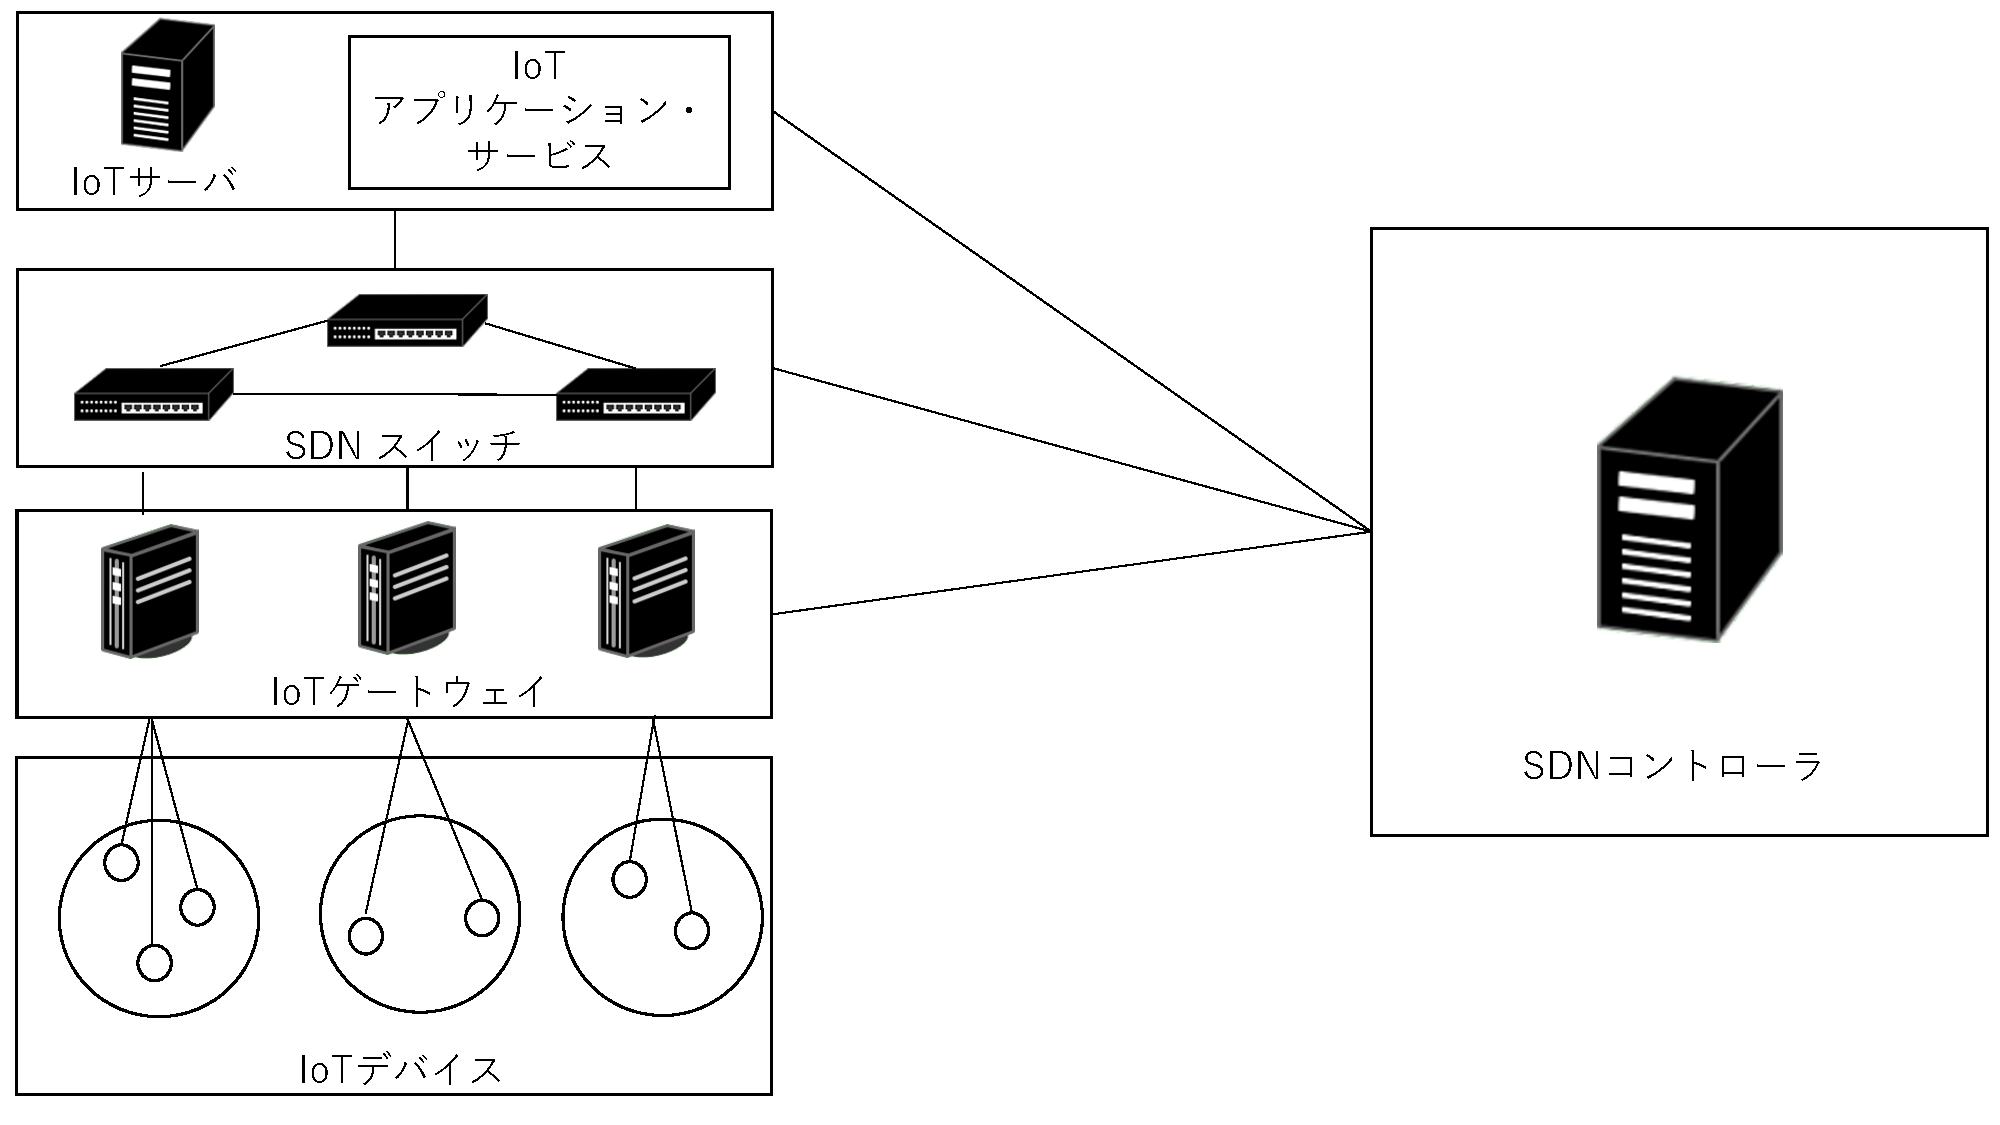
\includegraphics[width=\linewidth]{img/AQRA_Architecture.pdf}
  \caption{ネットワークトポロジ}
  \label{fig:Architecture}
\end{figure}

%---------------------------------------------------------------------
\section{まとめ}
本研究では,ホームネットワークのサービスを重要度やQoS要件,リアルタイム性から4つの優先度に分類し,アドミッション制御を行う.
リアルタイム性に着目することで,ドロップされた際のサービスへの影響を軽減した優先度制御を実現する.
各カテゴリの通信性能とドロップ間隔を測定し,サービスへの影響を考察し,提案手法の有効性を検証する.

%---------------------------------------------------------------------
% Bibliography
\footnotesize{
  \begin{thebibliography}{99}
    \bibitem{framework} Hung-Chin Jang, Chi-Wei Huang and Fu-Ku Yeh.Design A Bandwidth Allocation Framework for SDN Based Smart Home.\textit{2016 IEEE 7th Annual Information Technology, Electronics and Mobile Communication Conference (IEMCON)}, pp. 1-6, 2016.

    \bibitem{AQRA} Guo-Cin Deng and Kuochen Wang.An Application-aware QoS Routing Algorithm for SDN-based IoT Networking.\textit{2018 IEEE Symposium on Computers and Communications (ISCC)}, pp. 186-191, 2018.
  \end{thebibliography}
}

%---------------------------------------------------------------------
\end{document}
%---------------------------------------------------------------------
